\documentclass{article}
\usepackage{url}
\usepackage{hyperref}
\hypersetup{
    colorlinks=true,
    linkcolor=blue,
    filecolor=magenta,      
    urlcolor=cyan,
}
\usepackage{graphicx}


\newcommand{\BEASTVersion}{2.4.x}
\newcommand{\TracerVersion}{1.6}
\newcommand{\BabelVersion}{0.1.4}

\title{Language evolution with BEAST {\BEASTVersion}}

\author{Remco Bouckaert}

\begin{document}
\maketitle


In this tutorial, we perform a cognate alignment analysis in BEAST v\BEASTVersion\ \cite{beast}, and look into how to interpret the results.
This tutorial assumes you already have done one of the other tutorials, and are familiar with BEAUti, BEAST and Tracer, but if you are not, you may try to start with the Divergence dating tutorial, available from \url{http://beast2.org/tutorials/}.

For this tutorial, you need
\begin{itemize}
\item BEAST version \BEASTVersion, available from \url{http://beast2.org/}
\item Tracer version \TracerVersion, available from \url{http://tree.bio.ed.ac.uk/software/tracer/}
\end{itemize}

We will run through the following steps:
\begin{itemize}
\item{Install Babel package}
\item{Set up analysis in BEAUti}
\item{Run analysis with BEAST}
\item{Analyse using Tracer}
\end{itemize}

\section*{Install Babel package}
Make sure that you have the Babel version \BabelVersion\ package installed. 

To install Babel, it is easiest to start BEAUti (a program that is part of BEAST), and select the menu File/Manage packages. A package manager dialog pops up, that looks something like this:

\begin{center}
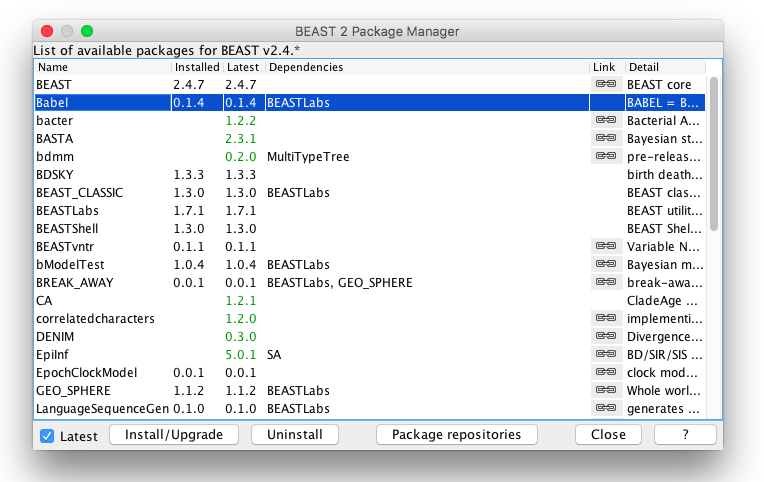
\includegraphics[width=0.75\textwidth]{package_manager.png}
\end{center}

If the Babel package is listed, just click on it to select it, and hit the Install/Upgrade button.

If the Babel package is not listed, you may need to add a package repository by clicking the "Package repositories" button. A window pops up where you can click "Add URL" and add "https://raw.githubusercontent.com/CompEvol/CBAN/master/packages-extra.xml" in the entry. After clicking OK, the dialog should look something like this:

\begin{center}
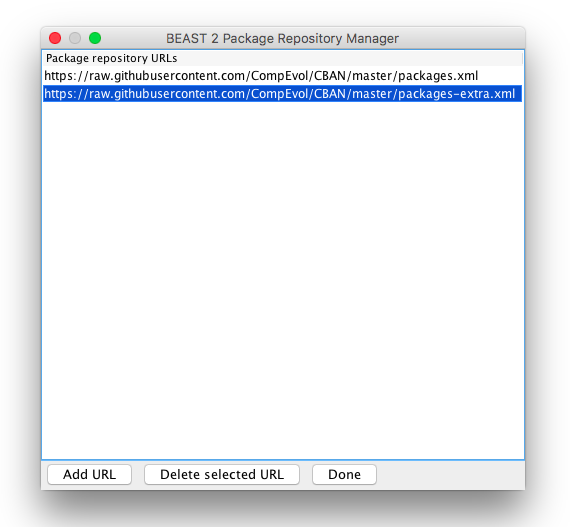
\includegraphics[width=0.75\textwidth]{package_repos.png}
\end{center}

Click OK and now Babel should be listed in the package manager (as in the first dialog above). Select and click Install/Upgrade to install.

Babel depends on the BEASTlabs package, which should be installed when you install Babel (unless it was already installed before).
See \url{http://beast2.org/managing-packages/} for details on how to install packages.

\section*{Set up analysis in BEAUti}

We will analyse an alignment of 24 languages  with 3014 sites + 1 ascertainment site collected by Ringe \cite{ringe2001}. 
When you install Babel, a number of cognate specific templates become available: 
\begin{itemize}
\item BinaryCTMC for using the CTMC model\cite{gray2003language,IE2013},
\item BinaryCovarion for using the covarion model\cite{tuffley1998modeling,IE2013,gray2009language}, and
\item SDollo for using the stochastic Dollo model\cite{nicholls2008dated,alekseyenko2008wagner,atkinson2005words}.
\end{itemize}
You find them under the File/Templates menu in BEAUti. We will perform a covarion analysis, so choose the BinaryCovarion template.

\begin{center}
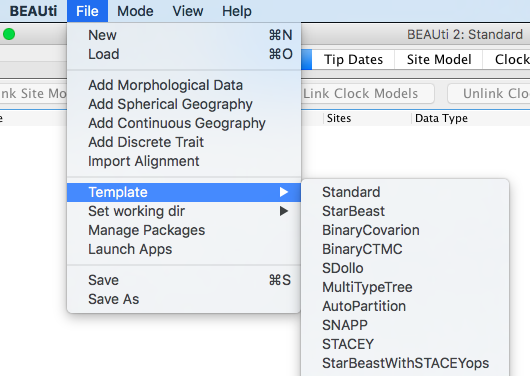
\includegraphics[width=0.75\textwidth]{templates.png}
\end{center}

Import the data, by selecting menu File/Import data, and select the file "ringe.nex".  

Hint: the "ringe.nex" file is part of the Babel package, and you can find it in the "examples/nexus" directory. The easiest way to navigate there is to select the menu File/Set Working Dir/Babel before selecting File/Import data.

This sets up the following:
\begin{itemize}
\item A single partition appears in the partition panel. This analysis uses the old style of ascertainment correction: it just assumes no site is all zeros, but ignores cases where there is missing data. Though we know this is not correct, it runs fast, so for the purpose of this tutorial it is more practical to just use this dodgy model.
\item There are ancient languages in the analysis, and the nexus file contains information on tips, so tips dates are set up.
\item There are some groupings known from the literature, and the nexus file contains these groupings. Monophyletic constraints are added accordingly.
\end{itemize}

\subsection*{Fix tip dates}

Click the tip-dates panel. It looks like the age for Umbrian was not correctly encode in the nexus file, so edit it and set it to 2200 year old. The other tip dates were (hopefully correctly) imported from the nexus file.

\begin{center}
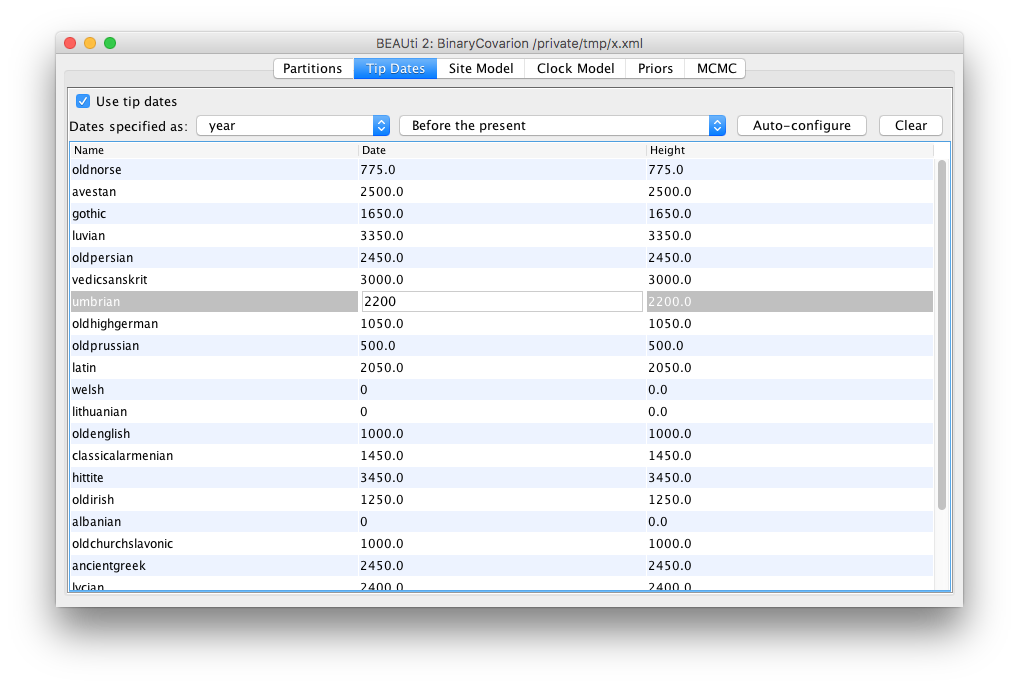
\includegraphics[width=0.99\textwidth]{tipdates}
\end{center}

\subsection*{Fix monophyly constraints}

Click the priors panel, which contains all constraints imported from the nexus file. There are age priors for tip dates of languages and for the internal nodes for Germanic and Tocharian (the ones with a Normal prior) and a monophyletic constraint for Anatolian (the ones with [none]).

\begin{center}
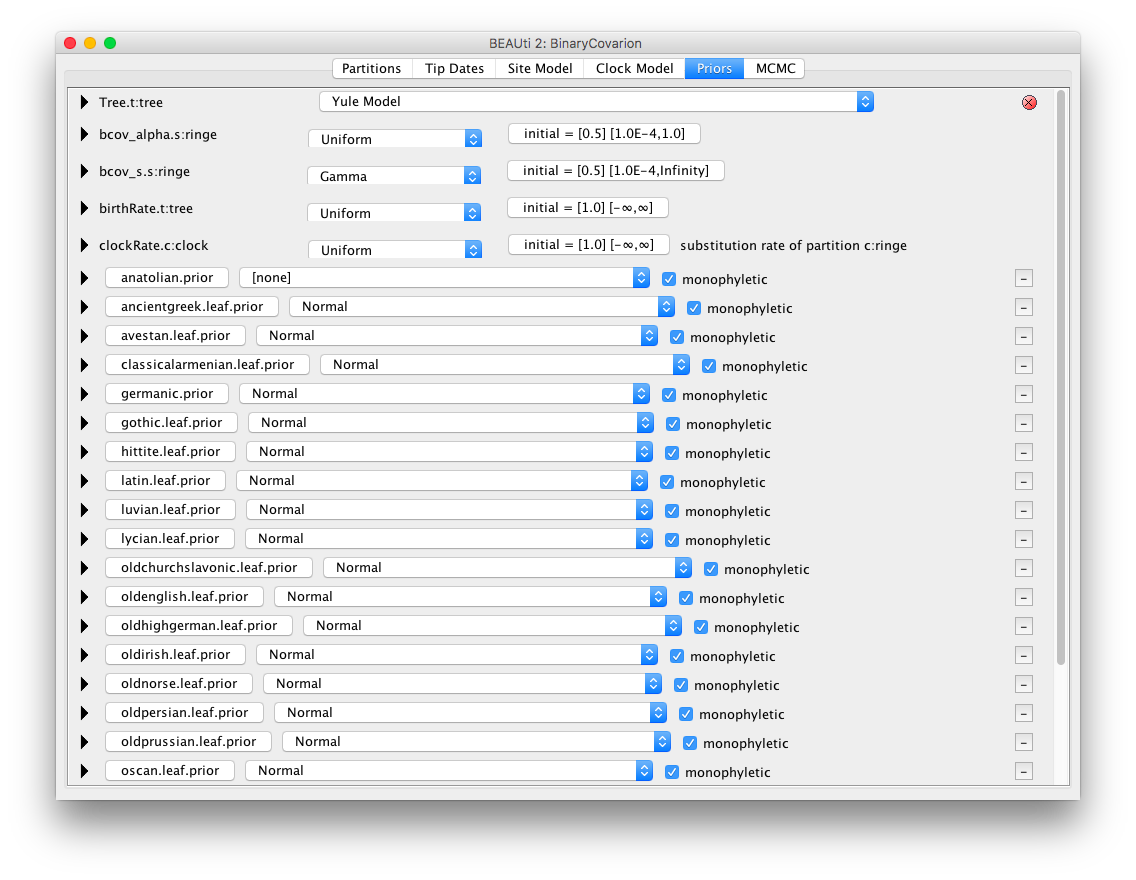
\includegraphics[width=0.99\textwidth]{priorpanel0}
\end{center}

Unfortunately, there is a mistake in the definition of Germanic; it contains Old Prussian, which is a Slavic language, so we need to remove it. Click the button labelled "Germanic" and deselect  OldPrussian, and only three languages should be left on the right hand side. Click OK to continue.

\begin{center}
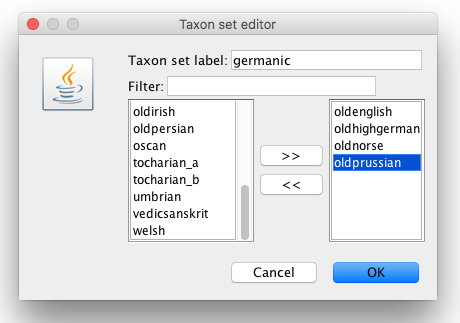
\includegraphics[width=0.49\textwidth]{germanic}
\end{center}

Another oversight is the lack of a tip prior for Umbrian. Scroll to the bottom of the priors panel, and click the "+ Add priors" panel. It is possible the following dialog pops up, where you select "MRCA prior".

\begin{center}
\includegraphics[width=0.49\textwidth]{MRCAPrior}
\end{center}
A new dialog pops up where you can specify taxon sets. In this case, we want to specify only a single taxon  in the set: select "umbrian" and add "Umbrian" under the taxon set label, and clock OK.
\begin{center}
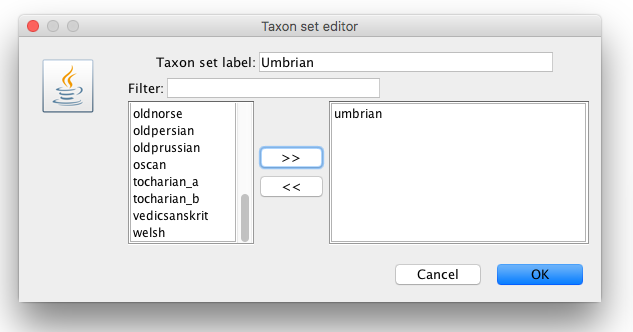
\includegraphics[width=0.49\textwidth]{umbrian}
\end{center}

In the priors panel, Umbrain.prior should now be listed. In the drop-down box showing '[none]' select 'Normal'.
Click the little triangle to specify details of the distribution. We want a mean of 2200 and sigma of 50 year.
Make sure to select the "Tipsonly" checkbox, which ensures the calibration applies to the tip only, and an appropriate operator is added to the analysis for doing proposals for the age of Umbrian.

\begin{center}
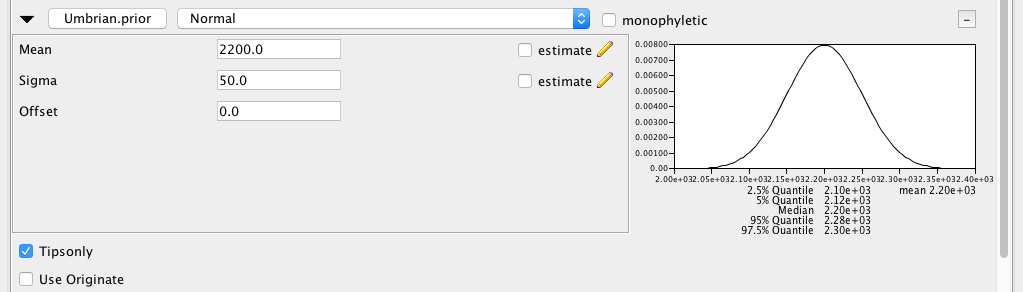
\includegraphics[width=0.49\textwidth]{umbrian2}
\end{center}

\subsubsection*{NEXUS}
Note that everything we did so far in BEAUTi could have been done by setting up the NEXUS file correctly and just importing that file.
This is how the alignment portion looks like. Note that the first column is all zeros. This first column is used for ascertainment correction by the templates in Babel (but not necessarily in any other templates).

\begin{center}
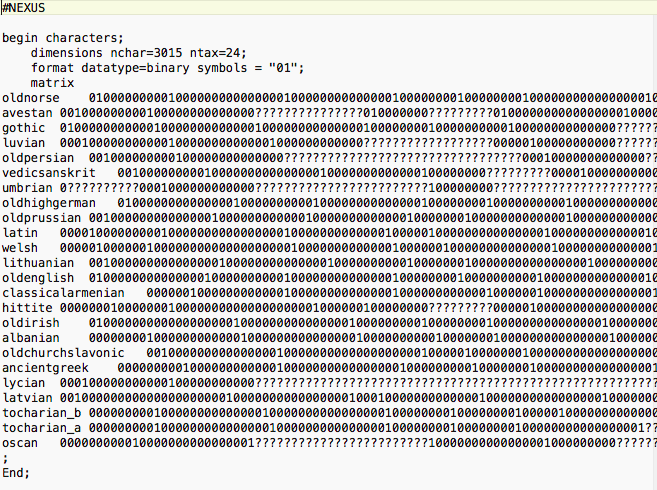
\includegraphics[width=0.9\textwidth]{nexus0}
\end{center}


{\bf Specify taxon sets}
For each clade ? group of taxa, like Germanic ? you need to specify a taxonset. The standard for this is to use a ?sets? block, and in the block all the taxon sets are specified. The format is 

\begin{verbatim}
begin set;
taxset <name1> = language11a language2a ? languagena;
taxset <name2> = language1b language2b ? languagenb;
... 
taxset <nameK> = language1K language2K ? languagenK;
end;
\end{verbatim}

Note the punctuation! There is a semi-colon at the end of each line, and taxon names are space delimited -- another reason not to have spaces in language names. Language names should refer to the languages present in the alignment. Each taxon set is assumed to be monophyletic, but you can change that in BEAUti of course.

{\bf Specify distributions.}
Distributions are specified in the ?assumptions? block.
Distributions can be specified over clades by referring to one of the taxon sets specified in the ?set? block above, or can contain a single (typically ancient) language, one of the languages specified in the alignment. The following distributions can be supported:

\begin{verbatim}
calibrate <node_name> = fixed(<age>)
calibrate <node_name> = uniform(<min_age>,<max_age>)
calibrate <node_name> = offsetexponential(<min_age>,<mean_age>)
calibrate <node_name> = normal(<mean_age>,<stdev>)
calibrate <node_name> = lognormal(<mean_age>,<stdev>)
calibrate <node_name> = offsetlognormal(<min_age>,<mean_age>,<stdev>)
calibrate <node_name> = gamma(<mean_age>,<stdev>)
calibrate <node_name> = offsetgamma(<min_age>,<mean_age>,<stdev>)          
\end{verbatim}

\begin{center}
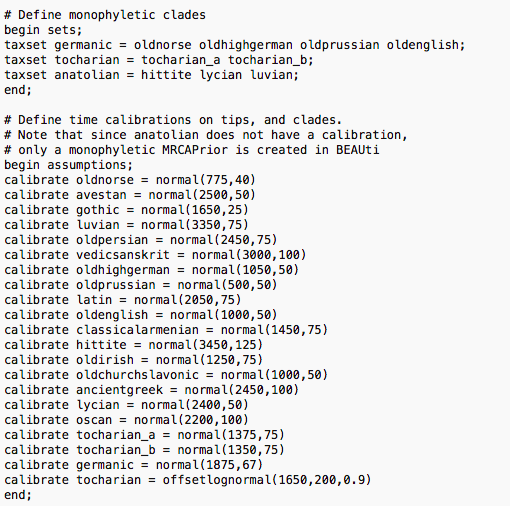
\includegraphics[width=0.9\textwidth]{nexus1}
\end{center}

{\bf Specifying partitions} To properly perform a cognate analysis, the meaning classes should be grouped, and each should get its own ascertainment column so that missing data is taken in account properly. For each meaning class, the first column should only contain zeros (if there is data for the meaning class) or question marks (if there is no data).
For each meaning class, a  'charset' command is added, which refers to the range of sites (including ascertainment site) for that meaning class. It looks something like this:

\begin{center}
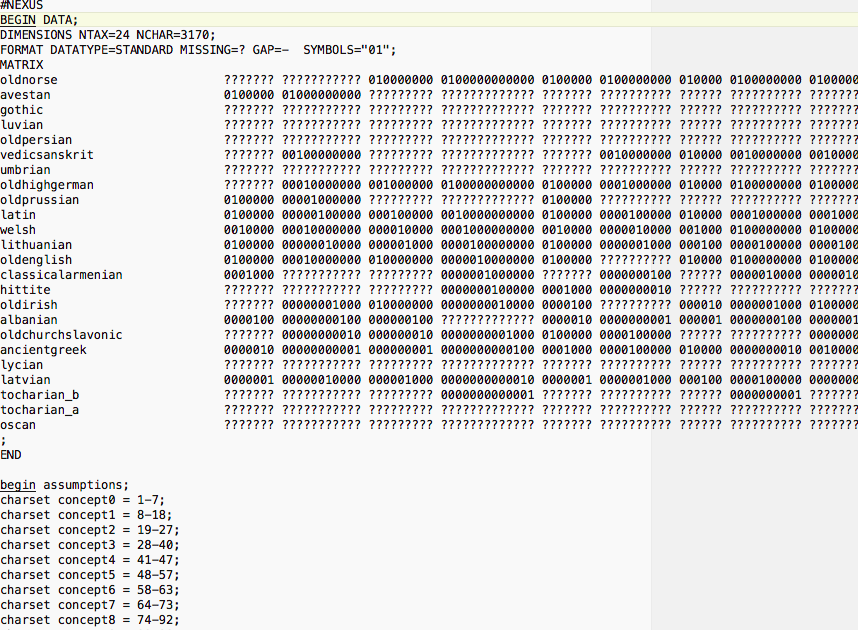
\includegraphics[width=0.9\textwidth]{nexus2}
\end{center}

When you import it in BEAUti with one of the Babel templates, the partition panel now shows one entry for each meaning class, but trees and clocks are automatically linked.

\begin{center}
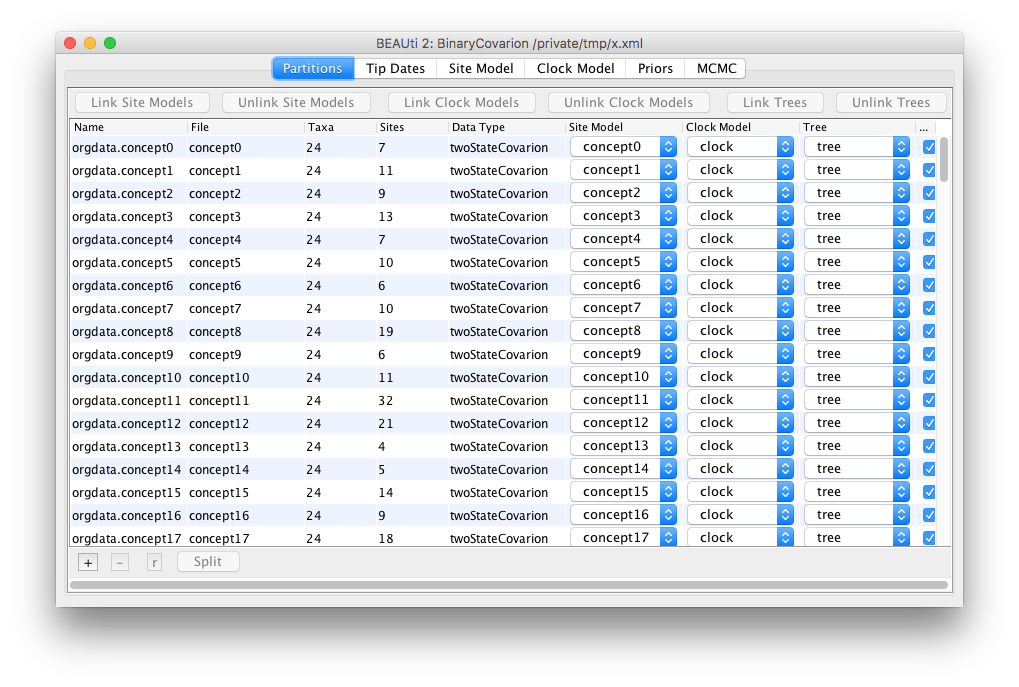
\includegraphics[width=0.99\textwidth]{partitionpanel}
\end{center}

\subsection*{Other priors}
The Yule prior (default) is only appropriate when all tips are contemporary.
Change it to the Bayesian Skyline Plot, which is a very flexible non-parametric coalescent prior. Usually, languages are considered similar to species, and birth/death/sampling models are used, but these are a bit harder to set up, so we go with the BSP for this tutorial.

There are priors for the clock model; make sure the clock rate has an upper bound of 1.0, otherwise it can escape to infinity.
Leave the prior for the standard deviation of the clock to its default value. 

\subsection*{Site model}
In the site panel, the relative mutation rate does not need to be estimated (since there is only 1 partition, the rate will remain fixed to 1 anyway), so the estimate box can be un-checked.

The hidden frequencies should not be estimated in BEAST mode, since it makes the model time irreversible. In REVERSIBLE and TUFFLYSTEEL mode they can be estimated. The Tuffly \& Steel model ignores the $\alpha$ parameter and assumes it is zero.

\begin{center}
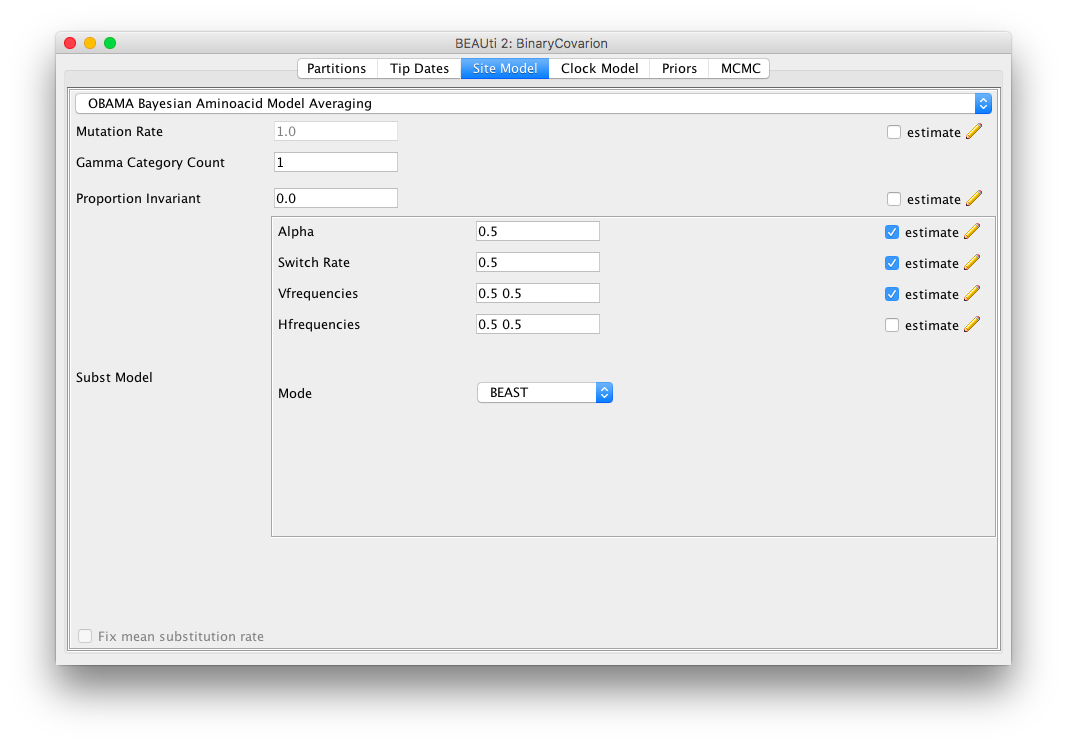
\includegraphics[width=0.75\textwidth]{sitepanel}
\end{center}

\subsection*{Change clock model}

In the clock model panel, change the clock from Strict clock to Relaxed clock with log normal distribution.
Thanks to the tip-dates, the mean clock rate will be estimated automatically.

\begin{center}
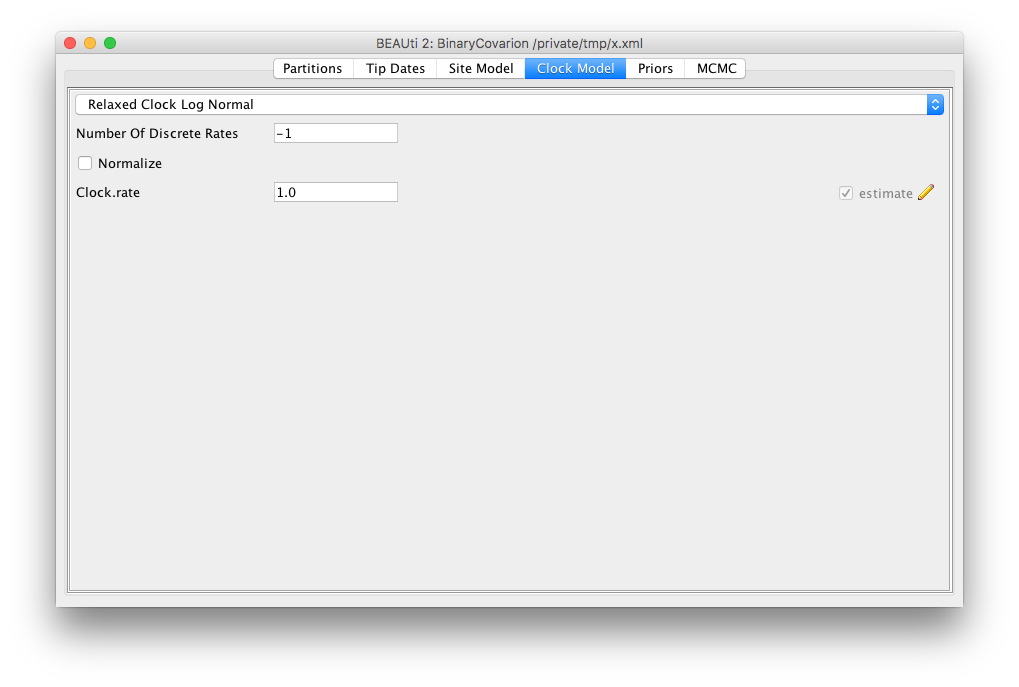
\includegraphics[width=0.75\textwidth]{clockpanel}
\end{center}

\subsection*{Change MCMC settings}

In the MCMC panel, change the chain length to 1 million and log frequencies to 10 thousand.

\begin{center}
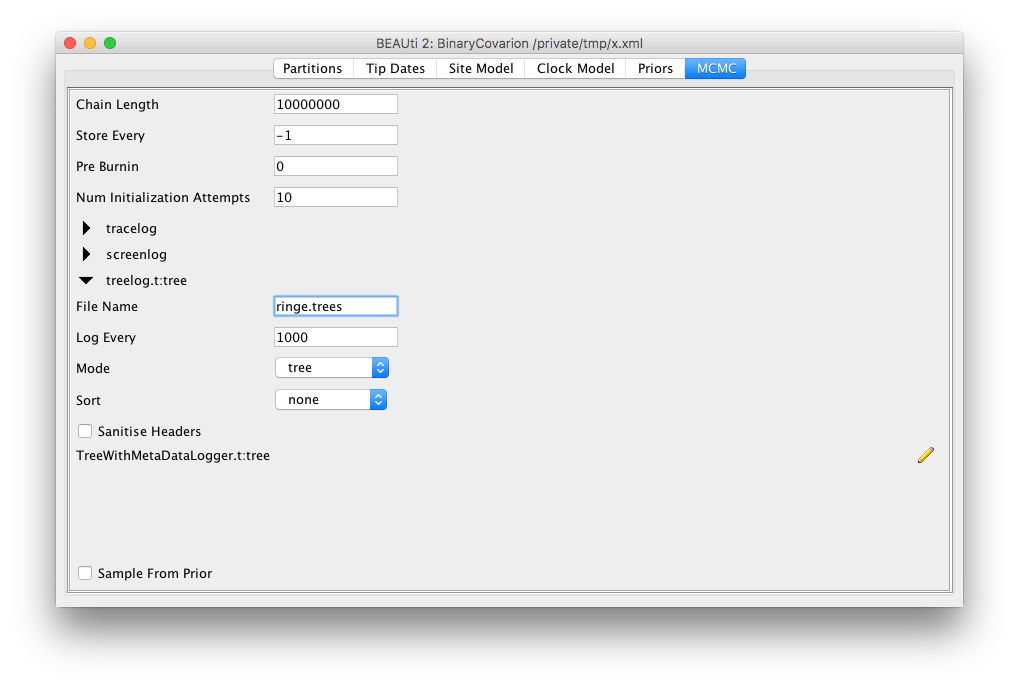
\includegraphics[width=0.75\textwidth]{mcmcpanel}
\end{center}

Save the file to say "ringe.xml" and now you are ready to run BEAST on the XML as usual.

\section*{Analysis}

As usual, check in Tracer that the analysis converged (or use the log files from \url{https://github.com/rbouckaert/Babel/releases/download/0.0.1/tutorial_data.zip}).

Does the tree distribution agree with what you know about Indo-European languages? Where did Old Prussian end up? What is the tip age of Umbrian?

What is the root age? How does this compare to the prior root age (you need to run the analysis with "Sample From Prior" checked in the MCMC panel, or edit the XML and addsampleFormPrior="true" on the run-tag)?

What does the tree prior look like in DensiTree? Can you identify the priors easily?

Do you think the prior root age is reasonable? If not, how would you change the root age? How does this affect the posterior?

\bibliographystyle{plain}
\bibliography{Babel}

\end{document}
